\begin{flushleft} \color{colorGris2}
	
	\section{Comandos rápidos}
	
	Ctrl + flechaDerecha: Cambia de opción en el editor TeXstudio.\newline
	
	Ctrl + clic: Lleva a la palabra que pertenece entre editor y el PDF.\newline
	
	\textbackslash indent: Inserta sangría.\newline
	
	\textbackslash noindent: Elimina sangría.\newline
	
	\textbackslash textbackslash: Inserta el carácter \textbackslash.\newline
	
	\textbackslash \%: Inserta el símbolo de porcentaje.\newline
	
	\textbackslash \$: Inserta el símbolo del dólar.\newline
	
	\textbackslash \#: Inserta el símbolo del numeral.\newline
	
	\textbackslash \&: Inserta el símbolo del and.\newline
	
	\textbackslash \_: Inserta el símbolo sub guion.\newline
	
	\section{Configuración del documento}
	
	Comando: \textbackslash documentclass[a4paper, 11pt]\{article\}\newline
	
	Acción: Configura el documento  a formato de hoja A4, con tamaño de texto 11pt en tipo de documento artículo.\newline
	
	\section{Entorno del documento}
	
	Comando: \textbackslash begin\{document\}\newline
	Aquí van los párrafos del documento.\newline
	\textbackslash end\{document\}\newline
	
	Acción: Todos los entorno empieza con Begin y terminan con end y el nombre del entorno entre corchetes.\newline
	
	\section{Paquete de colores}
	
	Comando: \textbackslash usepackage\{xcolor\}\newline
	\textbackslash definecolor\{rojo1\}\{rgb\}\{1.0, 0.03, 0.0\}\newline
	\textbackslash definecolor\{azul1\}\{rgb\}\{0.0, 0.75, 1.0\}\newline
	\textbackslash definecolor\{gris1\}\{rgb\}\{0.75, 0.75, 0.75\}\newline
	\textbackslash definecolor\{gris2\}\{rgb\}\{0.66, 0.66, 0.66\}\newline
	
	Acción: Sirve para configurar los colores que se utilizará en el documento.\newline
	
	\section{Paquete de fuentes}
	
	Comando: \textbackslash renewcommand*\textbackslash ttdefault\{lcmtt\}\newline
	\textbackslash renewcommand*\textbackslash familydefault\{\textbackslash ttdefault\}\newline
	\textbackslash usepackage[OT1]\{fontenc\}\newline
	
	Acción: Sirve para personalizar las fuentes del documento.\newline
	
	\section{Paquete de idioma}
	
	Comando: \textbackslash usepackage[spanish, es-nodecimaldot]\{babel\}\newline
	\textbackslash usepackage[utf8]\{inputenc\}\newline
	
	Acción: Sirve para indicarle a TeXstudio que estamos trabajando en el idioma español con la configuración utf8, el paquete de idiomas se llama babel, el parámetro es-nodecimaldot es para que el separador de decimales sea el punto y no  la coma.\newline
	
	\section{Secciones}
	
	Comando: \textbackslash section\{nombre de la sección\}\newline
	
	Acción: Sirve para generar secciones numeradas, si se desea que no  se vea el número, el comando  sería \textbackslash section*\{Secciones\} tener cuidado no ponerle asterisco a la primera sección.\newline
	
	\section{Índice}
	
	Comando: \textbackslash tableofcontents\newline
	
	Acción: Sirve para generar el índice, para actualizar el índice se debe compilar 2 veces.\newline
	
	\section{Salto de página}
	
	\subsection{Comando 1:} \textbackslash newpage\newline
	\subsection{Comando 2:} \textbackslash clearpage\newline
	
	Acción: Sirve para hacer saltos de páginas y para figuras y elementos flotantes se recomienda clearpage.\newline
	
	\section{Listas no numeradas}
	
	Comando: \textbackslash begin\{itemize\}\newline
	\textbackslash item hola1\newline
	\textbackslash item hola2\newline
	\textbackslash end\{itemize\}\newline
	
	Acción: Sirve para generar listas no numeradas, si se desea una sub lista se hace lo mismo de la lista y si se desea cambiar el símbolo del inicio de las líneas de las listas en los ítem sepone paréntesis así: \textbackslash item[-].\newline
	
	\section{Listas numeradas}
	
	Comando: \textbackslash begin\{enumerate\}\newline
	\textbackslash item hola1\newline
	\textbackslash item hola2\newline
	\textbackslash end\{enumerate\}\newline
	
	Acción: Sirve para generar listas enumeradas.\newline
	
	\section{Listas con descripción}
	
	Comando: \textbackslash begin\{description\}\newline
	\textbackslash item[Descripción 1] Esta es la descripción 1.\newline
	\textbackslash item[Descripción 2] Esta es la descripción 2.\newline
	\textbackslash end\{description\}\newline
	
	Acción: Sirve para generar listas con descripciones y estas generan sangrias si el texto es muy extenso.\newline
	
	\section{Figuras}
	
	Comando: \textbackslash usepackage\{graphicx\}\newline
	\textbackslash graphicspath\{\{./Figuras\}\}\newline
	
	Acción: graphicx sirve para cargar las figuras y graphicspath sirve para indicar la dirección de las figuras.\newline
	
	\begin{figure}[h]
		\centering
		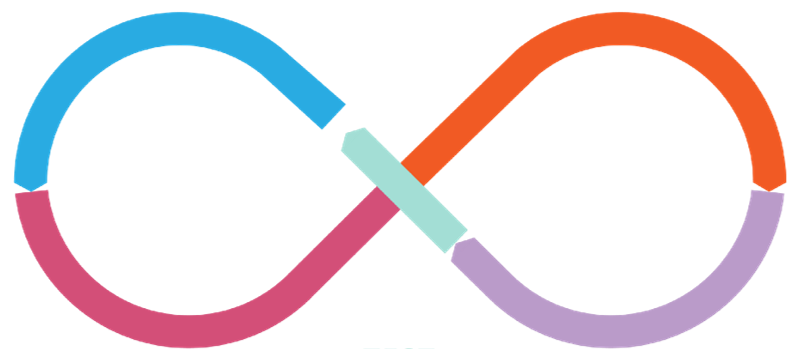
\includegraphics[width=0.25\textwidth]{flujo}
		\caption{Representación del infinito}
		\label{fig:flujo1}
	\end{figure}
	
	\begin{minipage}{0.99\textwidth}
		
		sfsdafa sagdgdf ggfdg gdfg gd gfdg gfgsgf ggsfg ggsdfg jhgjghjhk kjhgkhgkhg khgkhgkgh kjhkhkggkh khgkhgkh vxcvx cvxcv xcbcbvc bvcbv cbcvvnv nbmbn mnbmn bmn bmnb nbmnbmnb mn mnb mnbmbnmnb.
		
		\begin{wrapfigure}{l}{0.25\textwidth}
			\centering
			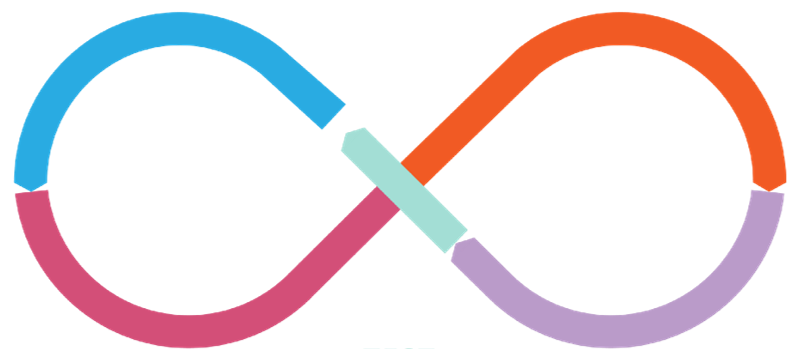
\includegraphics[width=0.9\linewidth]{flujo}
			\caption{Representación del infinito}
			\label{fig:flujo2}
		\end{wrapfigure}
		
		ggfdg gdfg gd gfdg gfgsgf ggsfg ggsdfg jhgjghjhk kjhgkhgkhg khgkhgkgh kjhkhkggkh khgkhgkh vxcvx cvxcv xcbcbvc bvcbv cbcvvnv nbmbn mnbmn bmn bmnb nbmnbmnb mn mnb mnbmbnmnb.
		
		sfsdafa sagdgdf ggfdg gdfg gd gfdg gfgsgf ggsfg ggsdfg jhgjghjhk kjhgkhgkhg khgkhgkgh kjhkhkggkh khgkhgkh vxcvx cvxcv xcbcbvc bvcbv cbcvvnv nbmbn mnbmn bmn bmnb nbmnbmnb mn mnb mnbmbnmnb.
		
		\begin{wrapfigure}{r}{0.25\textwidth}
			\centering
			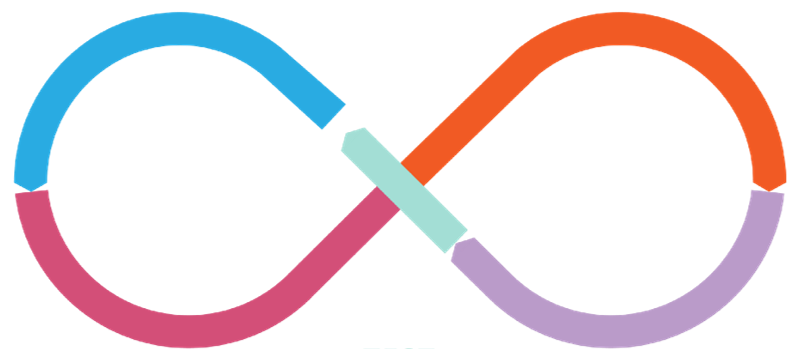
\includegraphics[width=0.9\linewidth]{flujo}
			\caption{Representación del infinito}
			\label{fig:flujo3}
		\end{wrapfigure}
		
		sfsdafa sagdgdf ggfdg gdfg gd gfdg gfgsgf ggsfg ggsdfg jhgjghjhk kjhgkhgkhg khgkhgkgh kjhkhkggkh khgkhgkh vxcvx cvxcv xcbcbvc bvcbv cbcvvnv nbmbn mnbmn bmn bmnb nbmnbmnb mn mnb mnbmbnmnb.
		
		dgdfgd gdffg sfdgfdgdfg gdfgdf
		
		ggfdg gdfg gd gfdg gfgsgf ggsfg ggsdfg jhgjghjhk kjhgkhgkhg khgkhgkgh kjhkhkggkh khgkhgkh vxcvx cvxcv xcbcbvc bvcbv cbcvvnv nbmbn mnbmn bmn bmnb nbmnbmnb mn mnb mnbmbnmnb.
		
		sfsdafa sagdgdf ggfdg gdfg gd gfdg gfgsgf ggsfg ggsdfg jhgjghjhk kjhgkhgkhg khgkhgkgh kjhkhkggkh khgkhgkh vxcvx cvxcv xcbcbvc bvcbv cbcvvnv nbmbn mnbmn bmn bmnb nbmnbmnb mn mnb mnbmbnmnb.
	\end{minipage}
	
	
	\section{Figuras que flotan}
	Ver en la imagen figura \autoref{fig:flujo4}.
	\begin{figure}[H]
		\centering
		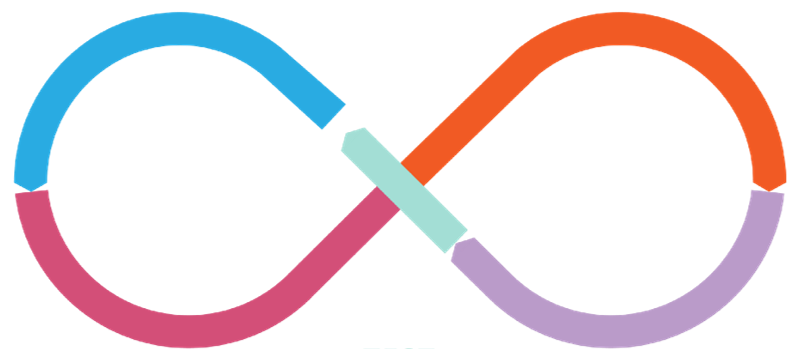
\includegraphics[width=0.6\linewidth]{flujo}
		\caption{Imagen sobre el infinito}
		\label{fig:flujo4}
	\end{figure}
	ggfdg gdfg gd gfdg gfgsgf ggsfg ggsdfg jhgjghjhk kjhgkhgkhg khgkhgkgh kjhkhkggkh khgkhgkh vxcvx cvxcv xcbcbvc bvcbv cbcvvnv nbmbn mnbmn bmn bmnb nbmnbmnb mn mnb mnbmbnmnb.
	
	
	\section{Dos figuras}
	ggfdg gdfg gd gfdg gfgsgf ggsfg ggsdfg jhgjghjhk kjhgkhgkhg khgkhgkgh kjhkhkggkh khgkhgkh vxcvx cvxcv xcbcbvc bvcbv cbcvvnv nbmbn mnbmn bmn bmnb nbmnbmnb mn mnb mnbmbnmnb.
	ggfdg gdfg gd gfdg gfgsgf ggsfg ggsdfg jhgjghjhk kjhgkhgkhg khgkhgkgh kjhkhkggkh khgkhgkh vxcvx cvxcv xcbcbvc bvcbv cbcvvnv nbmbn mnbmn bmn bmnb nbmnbmnb mn mnb mnbmbnmnb.
	
	\begin{figure}[h]
		\centering
		
\includegraphics[width=0.2\linewidth]{grafica_torta}
		\caption{La torta}
		\label{fig:torta1}
	\end{figure}
	
	\begin{figure}[h]
		\centering
		
\includegraphics[width=0.2\linewidth]{grafica_barras}
		\caption{Las barras}
		\label{fig:barra1}
	\end{figure}
	
	\begin{figure}[h]
		\centering
		\begin{subfigure}{0.45\textwidth}
			\centering
			
\includegraphics[width=0.4\linewidth]{grafica_torta}
			\caption{Una torta}
			\label{subtorta1}
		\end{subfigure}\hfil % Distribulle uniformemente las figuras y con hfill el espacio de enmedio se agranda
		\begin{subfigure}{0.45\textwidth}
			\centering
			
\includegraphics[width=0.4\linewidth]{grafica_barras}
			\caption{Unas barras}
			\label{subbarra1}
		\end{subfigure}
		\caption{Este es el caso donde se pueden poner 2 o más subfiguras la torta \ref{subtorta1} y las barras \ref{subbarra1}.}
		\label{fig:Dos subfiguras}
	\end{figure}
	
	ggfdg gdfg gd gfdg gfgsgf ggsfg ggsdfg jhgjghjhk kjhgkhgkhg khgkhgkgh kjhkhkggkh khgkhgkh vxcvx cvxcv xcbcbvc bvcbv cbcvvnv nbmbn mnbmn bmn bmnb nbmnbmnb mn mnb mnbmbnmnb.
	ggfdg gdfg gd gfdg gfgsgf ggsfg ggsdfg jhgjghjhk kjhgkhgkhg khgkhgkgh kjhkhkggkh khgkhgkh vxcvx cvxcv xcbcbvc bvcbv cbcvvnv nbmbn mnbmn bmn bmnb nbmnbmnb mn mnb mnbmbnmnb.
\end{flushleft}	


